\section{Qualitative Sensitivity Measures: the Morris Method}

This section introduces the Morris method for input screening.

\subsection{Input Screening}

In this section the applications of input screening is investigated.

% \begin{tabular}{lrr}
\toprule
{} &      $RC$ &  $\theta_{11}$ \\
\midrule
$RC$          &  1.604736 &       0.605903 \\
$\theta_{11}$ &  0.605903 &       0.273094 \\
\bottomrule
\end{tabular}


\subsection{Morris Method for Independent Inputs} \label{classic_morris}

The Morris method was introduced by \citet{M91} to identify the ``important" input variables of a model, especially in cases where there are many inputs and/or the evaluation of a model is time-consuming.

Consider the same setup as employed in the preceding sections. Let $x = \{x_1,\ \dots,\ x_k\}$ denote a sample of values assigned to the $X_i$'s. $f(x)$ is then the model output obtained for the values in $x$. Now consider a second sample $x_{\Delta_i} = \{x_1,\ \dots,\ x_{i-1},\ x_i + \Delta,\ x_{i+1},\ \dots,\ x_k\}$ that is identical to $x$ up to input $x_i$ which is varied by $\Delta$. Then, one elementary effect for input $i$ is derived by
\begin{equation}
EE_i = \frac{f(x_{\Delta_i}) - f(x)}{\Delta}.
\end{equation}

The above elementary effect is computed $N$ times, each for a varying $\Delta$ \citep{GM17}. The actual sm resulting from the Morris method are the mean, denoted by $\mu_i$, and the standard deviation, denoted by $\sigma_i$, taken from all $N$ different elementary effects per input $i$.
\begin{align}
\mu_i^\ast& = \frac{1}{N} \sum_{r=1}^N \vert EE_{i,\ r} \vert, \label{mu}\\
\sigma_i& = \sqrt{\frac{1}{N-1} \sum_{r=1}^N (EE_{i,\ r} - \mu_i)^2}, \label{sigma}
\end{align}

\noindent with $EE_{i,\ r}$ denoting the $r$-th elementary effect of input $i$, $r = 1,\ \dots, N$, and $\vert \cdot \vert$ the absolute value. Note that in \citet{M91} the absolute value was absent and elementary effects could potentially cancel each other out \citep{CCS07}. Therefore, \citet{CCS07} proposed the version presented above, thus making the screening method more robust. A total of $2 \cdot k \cdot N$ model evaluations is needed to compute the full set of sm using the Morris method.

$\mu_i^\ast$ and $\sigma_i$ can now be used to identify non-influential model inputs. Uninfluential inputs exhibit a $\mu_i^\ast$ close to zero. If $\mu_i^\ast$ is large, it depends on $\sigma_i$ whether there exist substantial non-linear or interaction effects. A low $\sigma_i$ indicates that non-linear effects are non-existent, whereas a high $\sigma_i$ suggests large interaction or non-linear effects \citep{GM17}.

The Morris method exhibits some drawbacks. Firstly, as they stand, the sensitivity indices derived by the Morris method are not suited for screening inputs under dependence. To see why consider two inputs $X_i$ and $X_j$ which are dependent, i.e. $G(x_i,\ x_j) \neq G(x_i)G(x_j)$, where $G(\cdot)$ again denotes the cumulative distribution function. If $x_i$ changes, $x_j$ should change as well due to the dependence between the two inputs. The sensitivity indices presented above are derived using a One-At-a-Time approach that does not allow for the screening of dependent inputs \citep{GM17}.

Secondly, similar to the Sobol' indices, the person conducting sa has to take two indices per input into account. Compare to the arguments made in \cref{var_based_sa}.

Thirdly, there exists no clear interpretation of the absolute values of the sensitivity indices. They only provide a ranking of inputs and give a hint of which inputs are the least influential ones \citep{GM17}.

On the advantages, Morris indices are easily computed, with a much lower computational burden than the Shapley effects as presented in \cref{comp_shap}. Recall that Shapley effects as computed by use of the algorithm in \citet{SNS16} came at a cost of $N_V+m \cdot N_I \cdot N_O \cdot (k-1)$ model evaluations. Even the more efficient approach by \citet{PRB20} needed $2^k$ model runs. See \cref{comparison} for a discussion of the respective computational costs.

Considering the interpretation of Morris indices, $\mu_i^\ast$ and $\sigma_i$, it is apparent that not only an input ranking is feasible but we can also learn something about the underlying model structure, i.e. whether interaction or non-linear effects are present.

\citet{M91} points out that his method does not rely on simplifying assumptions, e.g. monotonicity of the model or input sparsity. He argues that if those assumptions hold, one could apply other, more effective and economical procedures, e.g. based on Latin hypercube designs. However, the Morris method does not rely on such assumptions and will work well if these assumptions are justifiable or not \citep{M91}.

\citet{BP16} group the Morris method to the family of local sm. However, while the elementary effects themselves consider only local changes, the actual measures for input importance, $\mu_i^\ast$ and $\sigma_i$, average over these $N$ elementary effects. Thus, they take $N$ local changes per input $i$ into account \citep{M91}. Indeed, \citet{CCS11} make a case for the Morris method to be seen a global sm. \citet{BP16} acknowledge that screening methods like the Morris sm stand apart from other local sm.

\subsection{Algorithm for Extended Morris Method}

\begin{figure}[t]
	\caption{Convergence of Morris Indices}
    % \floatfoot{A note}
    \label{morris_convergence}
	\vspace*{-4mm}
	\centering
	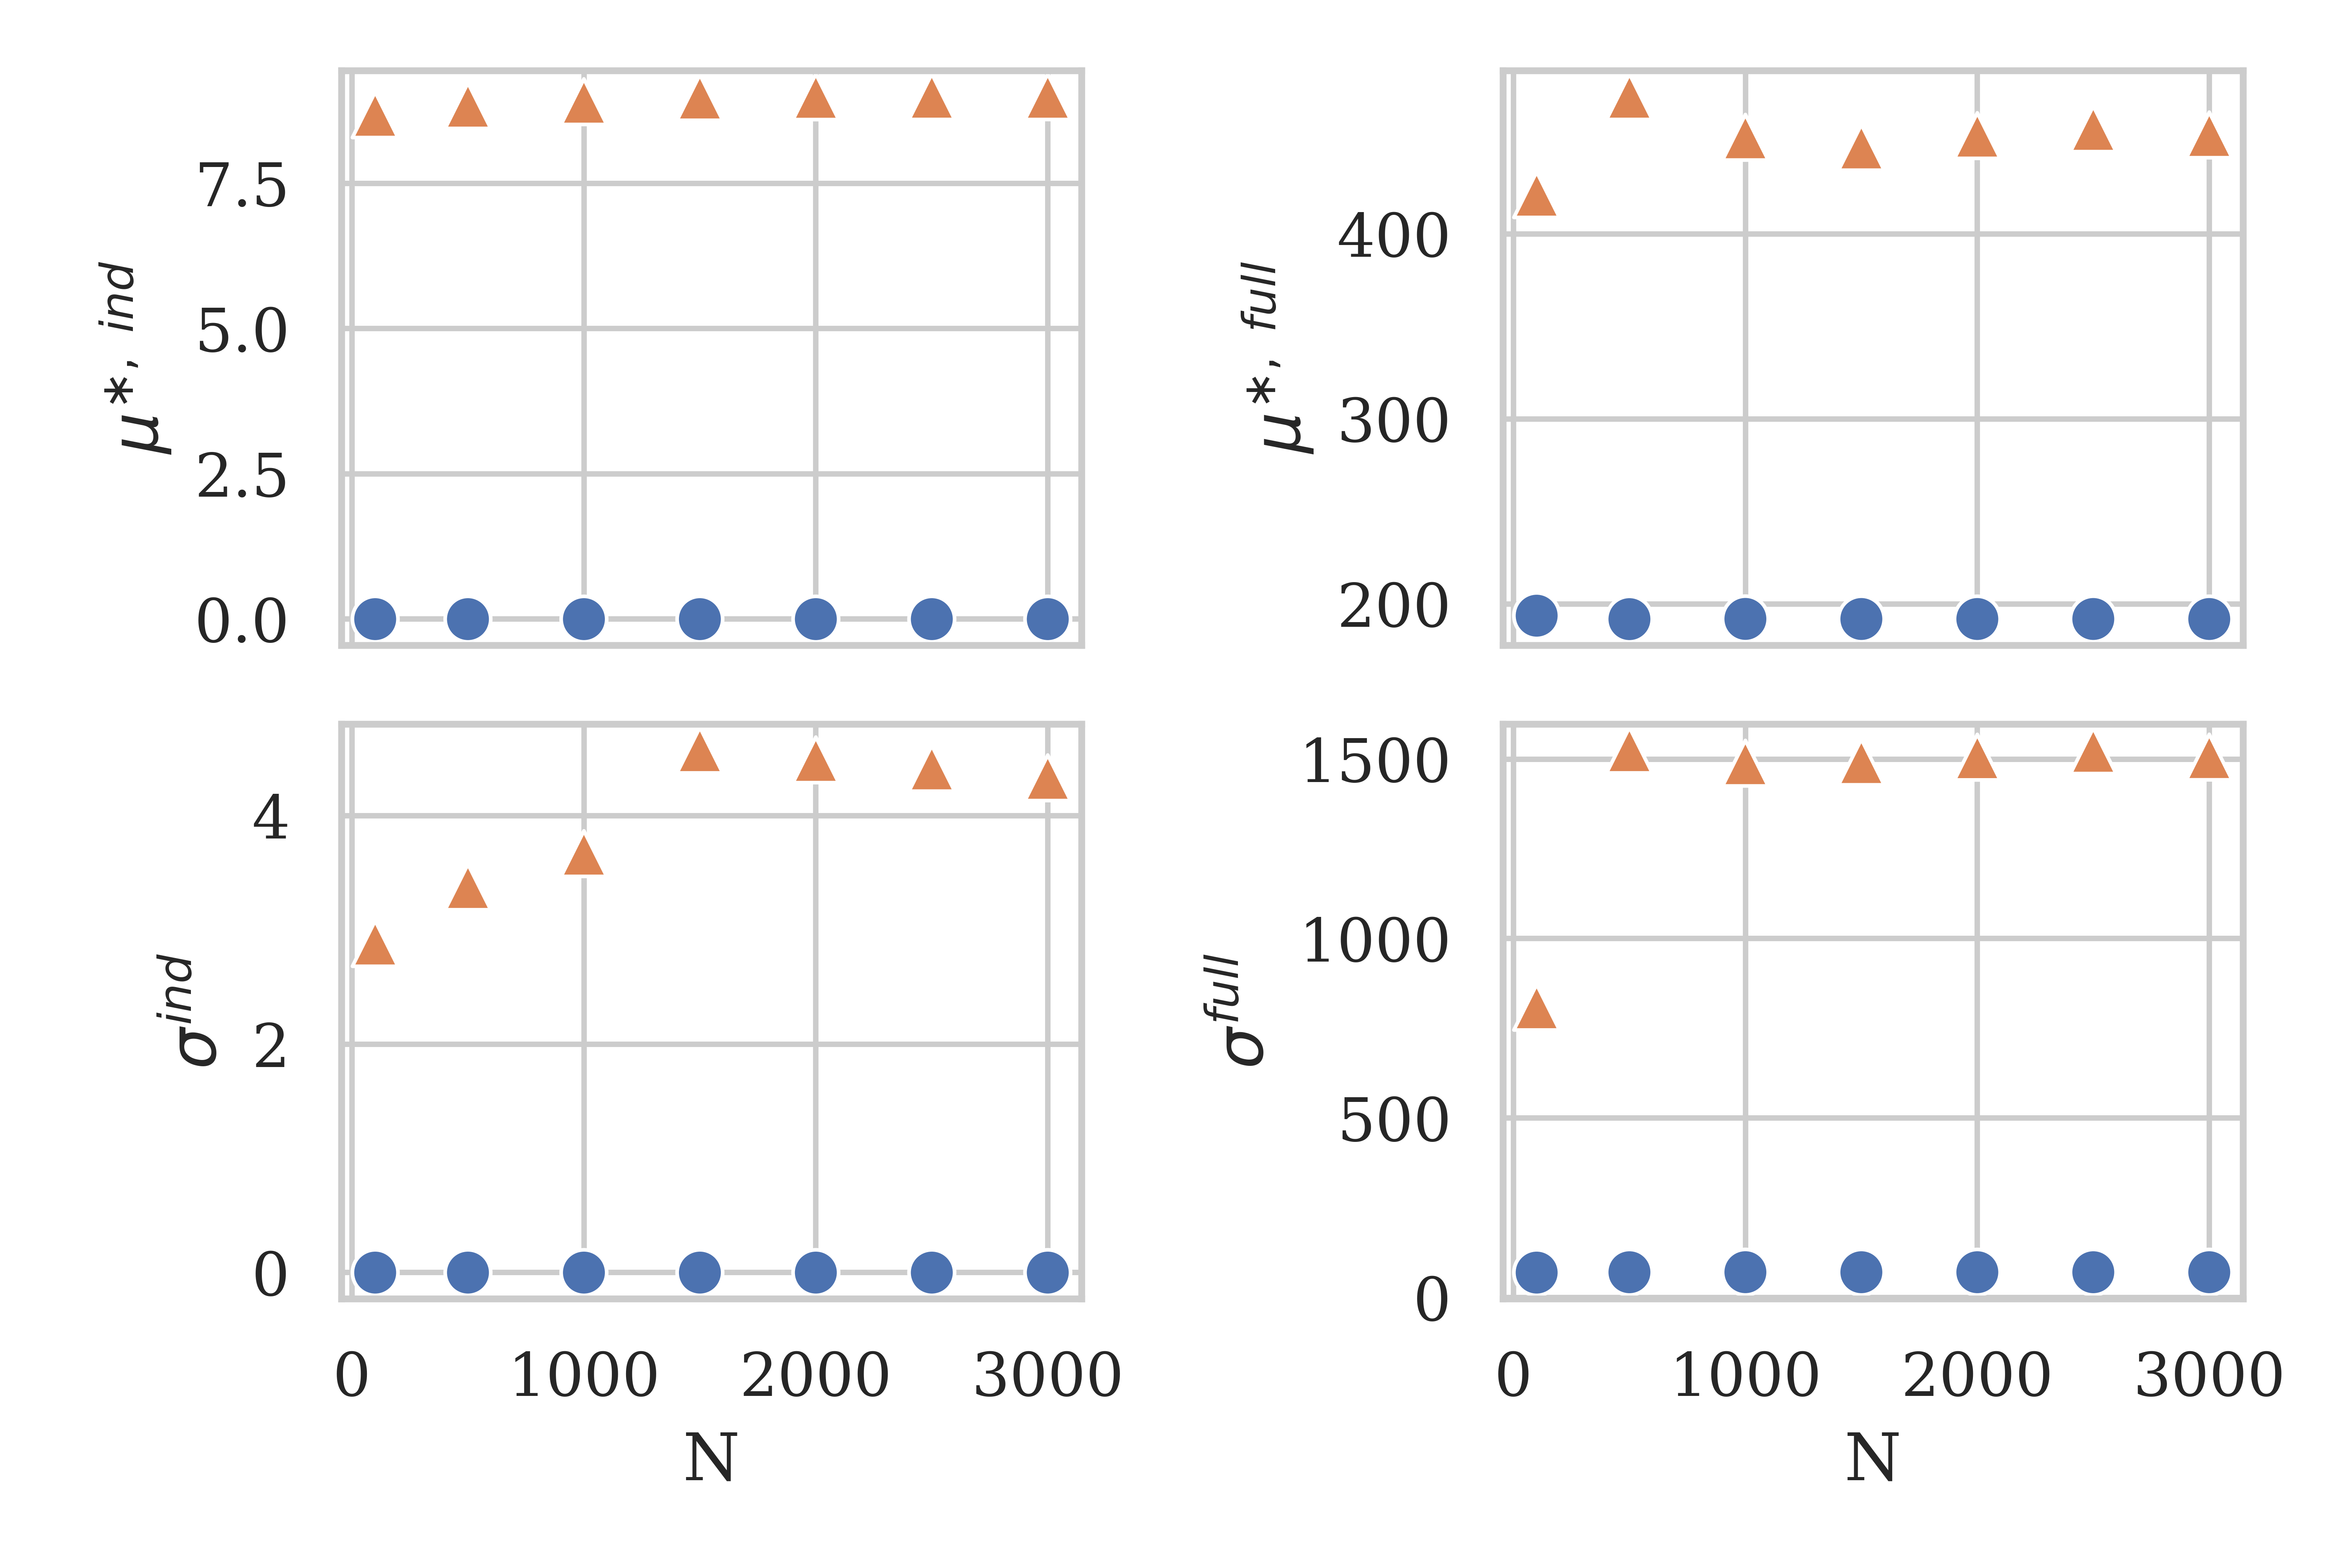
\includegraphics[scale=0.9]{../figures/morris_convergence.png}
\end{figure}

\begin{figure}[t]
	\caption{Uncertainty in Morris Indices - 100 Replicates}
    % \floatfoot{A note}
    \label{morris_replicates}
	\vspace*{-4mm}
	\centering
	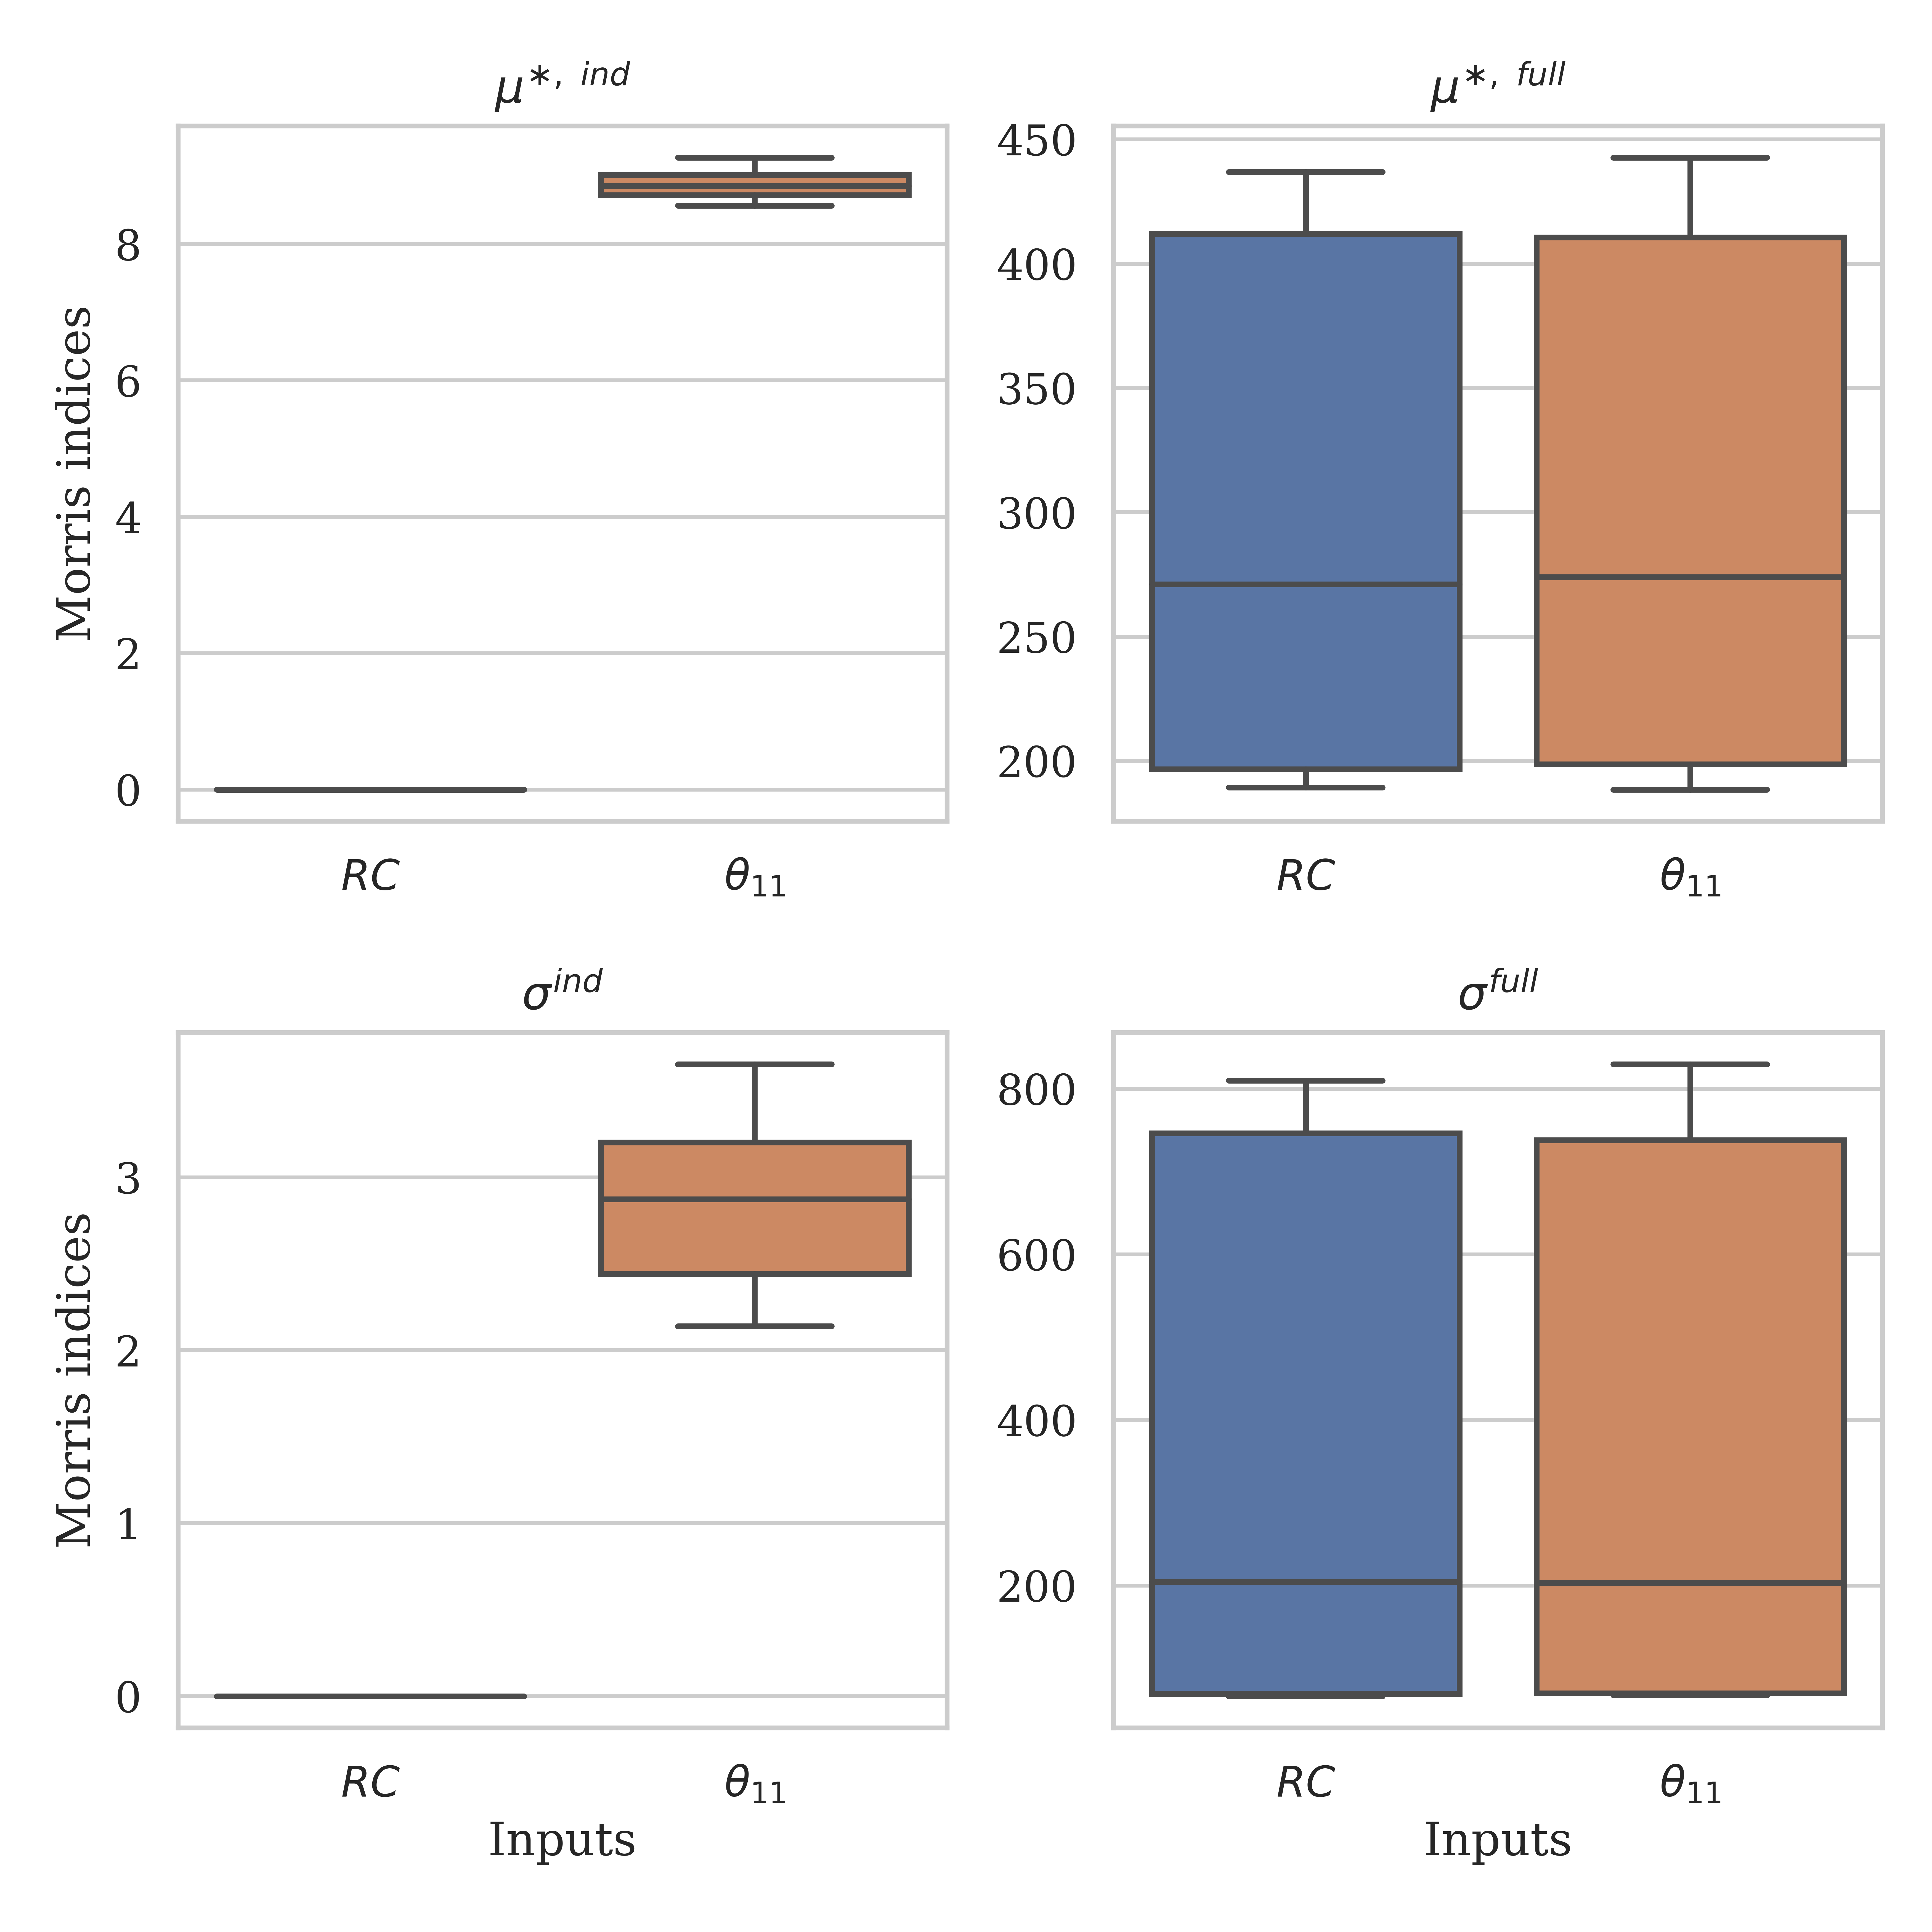
\includegraphics[scale=0.9]{../figures/boxplot_morris_replicates_100.png}
\end{figure}

In this section I introduce the extended Morris method for dependent samples as proposed by \citet{GM17}.

To grasp the computation procedure of the extended elementary effects, some more notation is needed. Following \citet{GM17}, let $X' = \{X_1',\ X_2',\ \dots,\ X_k'\}$ be $k$ dependent random inputs, following the joint pdf $g(X)$. Thus, $X'$ is just a set of inputs independently drawn from the set $X$. Input subsets denoted by $\bar{X}$ are conditionally drawn inputs. Hence, let $\bar{X_{-i}'}$ follow the conditional pdf $g(\bar{X_{-i}'} \mid X_{-i})$. That is $\bar{X_{-i}'}$ is drawn conditionally on the inputs in the first set $X_{-i}$. The input denoted by $\bar{X_{-i}}$ is conditionally drawn following the pdf $g(\bar{X_{-i}} \mid X_i')$. % Hence, $\bar{X_{-i}'}$ and $\bar{X_{-i}}$ differ by [].

Analogously to the independent and full Sobol' indices \citep{MTA15}, \citet{GM17} developed the following elementary effects for dependent inputs.
\begin{align}
EE_i^{ind} = \frac{f(\bar{x_i}',\ x_{-i}) - f(x_i,\ x_{-i})}{\Delta},\\
EE_i^{full} = \frac{f(x_i',\ \bar{x_{-i}}) - f(x_i,\ x_{-i})}{\Delta},
\end{align}

\noindent where
\begin{itemize}
\item $EE_i^{ind}$ denotes \textit{independent} elementary effects for input $i$, effects that exclude the contributions attributable to the dependence between input $X_i$ and $X_j$ for $i \neq j$, and
\item $EE_i^{full}$ denotes \textit{full} elementary effects for input $i$, that include the effects due to correlation with other inputs.
\end{itemize}

As in the case of the classic Morris method, the sm for input $i$ is derived by considering $N$ random samples yielding $2 \cdot N$ elementary effects, once for the independent and once for the full elementary effects. \citet{GM17} compute the corresponding sm as shown in \cref{mu} and \cref{sigma}. Since two sets of elementary effects are computed, they end up with a set of four sm, $(\mu^{\ast ind}_i,\ \sigma_i^{ind})$ and $(\mu^{\ast full}_i,\ \sigma_i^{full})$.

Interpretation-wise, $X_i$ is an unimportant input if all sm are essentially zero. A $\mu^{\ast ind}_i$ strongly larger than zero and $\sigma_i^{ind}$ is close to zero, input $X_i$ is an important input by itself. When all sm except $\mu^{\ast full}_i$ are close to zero, $X_i$'s contribution is due to the dependence with other important inputs. Strong interaction effects are present if either or both of the two $\sigma$'s is larger than zero \citep{GM17}.

The computation of the extended Morris indices requires the generation of dependent samples. According to \citet{GM17}, the computation involves the following steps:

\begin{enumerate}
    \item Create independent, uniformly distributed samples.
    \item Transform these uniformly distributed samples into dependent samples of a target distribution.
    \item Use the above methods for the computation of the extended elementary effects.
    \item As in the case of the classic Morris method, average over all $N$ elementary effects per input $i$ and compute their standard deviation. Do so for the \textit{independent} and \textit{full} elementary effects.
\end{enumerate}

In what follows I stick to the version of the algorithm as implemented in the \textit{econsa} Python-package \citep{OSE21}. There, the radial design is used for obtaining independent samples. To derive dependent samples, the inverse Nataf transformation is applied. The total computational cost amounts to $3kN$ model runs.

\subsection{Morris Indices for the Rust Model} \label{morris_rust_model}

I estimate Morris indices in two different ways, similar to the procedure described in \cref{comp_shap}: i. I estimate 100 replicates for a relatively low sample size to get a sense of the variability in estimates and ii. I consecutively increase the sample size to investigate
the estimation procedure further. Uniformly distributed samples are drawn from a Sobol'
sequence \citep{S76}.

Firstly, I estimate 100 sets of Morris indices. In order to ensure comparability, I use the same total computational cost as for the data used for \cref{boxplot_shapley}. I set $N = 27$, which amounts
to a total cost of 162 model evaluations, which differs slightly from the computational
cost for the Shapley effects because of rounding. As stated above, there are four different
sensitivity indices estimated: $(\mu^{\ast ind}_i,\ \sigma_i^{ind})$ and $(\mu^{\ast full}_i,\ \sigma_i^{full})$. The distribution of the
estimated Morris indices is given in \cref{morris_replicates}.

Inspecting \cref{morris_replicates}, we can get a sense of the uncertainty in the estimation procedure,
given the admittedly small sample size. For the independent Morris indices, there exists a
very clear ranking: both values indicate that $RC$ is uninfluential. For $\theta_{11}$ the situation is
different: both independent indices are nonzero. Surprisingly, for the full Morris indices,
we fail to observe a clear input ranking. Estimates of $(\mu^{\ast full}_i,\ \sigma_i^{full})$ are very volatile, but
clearly different from zero. Interpretation-wise, this may seem as a challenge, since no
clear input ranking is achieved. But in fact, it is not. Morris indices were perceived to
identify non-influential inputs. Both inputs are important if the full Morris indices are
considered.

To investigate whether the individual pairs of full Morris indices, $(\mu^{\ast full}_i,\ \sigma_i^{full})$, for the
two inputs $i \in \{RC,\ \theta_{11}\}$ yield the correct input ranking, I simply compare their values
per estimate. Surprisingly, xy of the 100 replicates yield the correct importance ranking
for $\mu^{\ast full}_i$. Regarding $\sigma_i^{full}$, xy out of 100 replicates successfully identify $\theta_{11}$ as the more
important input.

\begin{table}
    \caption{Relative Difference in Morris Indices}
    \label{rel_diff_morris}
\end{table}

\begin{table}
    \caption{Morris Indices for $N=3,000$}
    \label{morris_3000}
\end{table}

Secondly, I estimate Morris indices for a set of number of draws. I consider $N \in \{100,\ 500,\ 1000,\ 1500,\ 2000,\ 2500,\ 3000\}$. Results are shown in \cref{morris_convergence}. Morris indices in
\cref{morris_convergence} clearly confirm the input ranking of the replicates as presented above. Morris indices
converge as $N$ increases. \Cref{rel_diff_morris} confirms this. Although Morris indices are volatile, \citet{GM17} point out that a high estimation precision is not necessarily needed
as long as the input ranking is clearly achieved.
Let us inspect the Morris indices for $N = 3,000$ in more detail. Consult \cref{morris_3000} for the
resulting Morris indices. The computational cost for this value of $N$ amounts to $18,000$
model evaluations. If only the independent Morris indices are considered, we erroneously
conclude that input $RC$ is a non-influential input. [More interpretation. As in GM17.
What ca we learn about the structure of the model!?]
